\documentclass[12pt]{article}

% Packages
\usepackage{graphicx}
\usepackage{amsmath}
\usepackage{geometry}
\geometry{margin=1in}
\usepackage{float}
\usepackage{caption}
\usepackage{subcaption}
\usepackage{cite}
\usepackage{parskip}

\title{ME155C Final Project Report\\Inverted Pendulum Control: Swing-up, Balance, and Catching}
\author{Raaghav Thirumaligai, Cole Giusto, Tien Nguyen}
\date{June 8, 2025}

\begin{document}

\maketitle

\begin{abstract}
This project focuses on the identification, modeling, and control of an inverted pendulum on a cart system. Through experimental identification, control design, and closed-loop testing, we implemented robust swing-up, balancing, and catching controllers. System identification methods included logarithmic sine sweeps and parametric identification with MATLAB's tfest. Controller design employed energy-based swing-up methods and robust LQR/LQG balancing strategies. Experimental validations confirm effective performance, achieving stable equilibrium transitions and pendulum catching.
\end{abstract}

\section{Introduction}
This project investigates the control of an inverted pendulum on a cart, specifically targeting swing-up, balancing, and catching tasks. The inverted pendulum, a classic control problem, requires precise and robust feedback control strategies due to its inherent instability. Previous literature includes methods involving energy-based swing-up and state-space feedback stabilization. The report is structured with system identification in Section 2, controller design in Section 3, closed-loop results in Section 4, and conclusions in Section 5.

\section{System Identification}

\subsection{Process Description}
The experimental setup consists of an asymmetric metal rod mounted to a motor-driven cart, with encoders providing measurements of pendulum angle ($\theta$) and cart position ($x$). The control input is the motor voltage ($u$), and the primary controlled outputs are cart position and pendulum angle.

\begin{figure}[H]
    \centering
    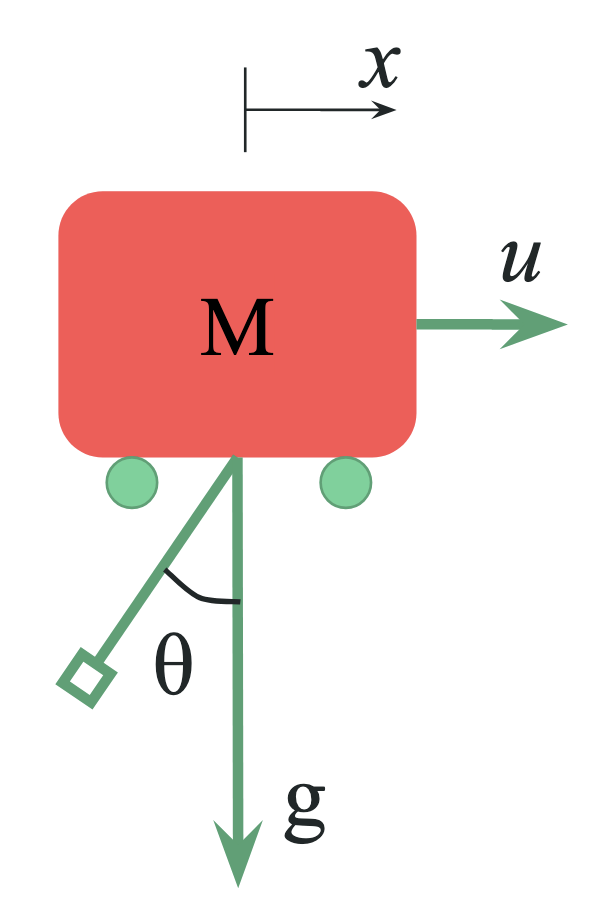
\includegraphics[width=0.15\textwidth]{figures/system_setup.png}
    \caption{Experimental setup: Cart-pendulum system.}
    \label{fig:setup}
\end{figure}

\subsection{Identification Methods}

Non-parametric identification utilized a logarithmic sine sweep ($0.3-3$ Hz). Parametric identification was done using MATLAB's \texttt{tfest} function, performing 30 experimental trials.

\begin{figure}[H]
    \centering
    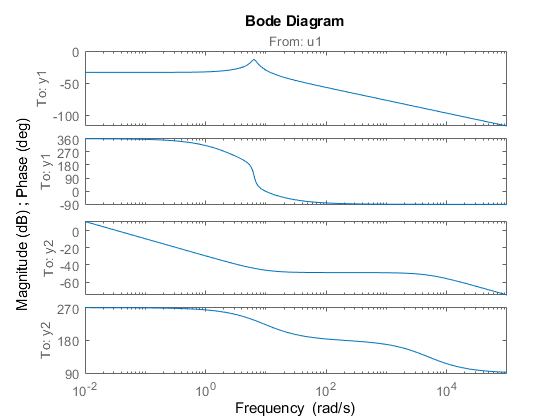
\includegraphics[width=0.8\textwidth]{../plots/bode_down.png}
    \caption{Bode plot: Identified frequency response for cart dynamics and pendulum dynamics downwards.}
    \label{fig:bode_down}
\end{figure}

\begin{figure}[H]
    \centering
    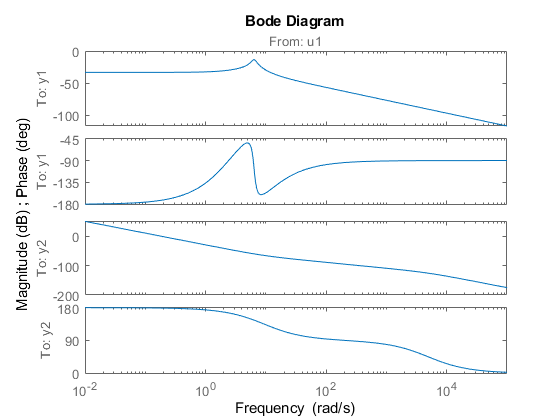
\includegraphics[width=0.8\textwidth]{../plots/bode_up.png}
    \caption{Bode plot: Identified frequency response for cart dynamics and pendulum dynamics upwards.}
    \label{fig:bode_up}
\end{figure}


\section{Controller Design}

\subsection{Swing-Up Controller}
The swing-up controller uses an energy addition method to drive the pendulum toward the upright position.
Around every zero crossing of the pendulum angle $\theta$, the controller applies a force to move the cart in the direction opposite to the pendulum's velocity in order to increase the energy in the pendulum.
This continues until the pendulum is able to fully ``swing up''.
Additionally, a simple proportional controller is used to regulate the cart's position to stay near zero meters, preventing excessive cart movement during the swing-up phase.
The activation is limited to a range $\theta \in [-30^\circ,30^\circ]$ to try and reach the inverted state with a small velocity.


\begin{figure}[H]
    \centering
    
\includegraphics[width=0.6\textwidth]{figures/ph.png}
    \caption{Swing-up controller activation.}
    \label{fig:swingup}
\end{figure}

\subsection{Balancing Controller}
The balancing controller employs LQR/LQG methods to stabilize the pendulum in the inverted (unstable) equilibrium within a narrow angular region. 
First, we created an LQR controller to properly penalize the relevant states and try to achieve the best performance. 
The $Q$ matrix was tuned to aggressively control the pendulum angle but allow the cart to move relatively freely. 
This allowed the system to use large cart movements to stabilize the equilibrium and stay in the linear regime.
\begin{align*}
    Q = \begin{bmatrix}
        2000 & 0 & 0 & 0 \\
        0 & 20 & 0 & 0 \\
        0 & 0 & 10 & 0 \\
        0 & 0 & 0 & 0.01
    \end{bmatrix}
\end{align*}
The columns correspond to the states: angular position, angular velocity, cart position, and cart velocity respectively.

For the LQG state estimation to feed into the LQR controller, we used a Kalman filter block in Simulink. 
With the default settings, feeding in our output and input signals, the Kalman filter was able to reliably provide an
accurate estimate of the state to the controller.


\subsection{Catching Controller}
Similar to balancing, catching employs LQR/LQG but aims to return the pendulum reliably to the stable downward equilibrium.

\subsection{State Machine}
Control modes transition between swing-up, balancing, and catching using a robust state machine architecture.
This state machine was implemented in Simulink using logic gates, comparing the pendulum angle and velocity to determine the current state and enable the correct controller.

\begin{figure}[H]
    \centering
    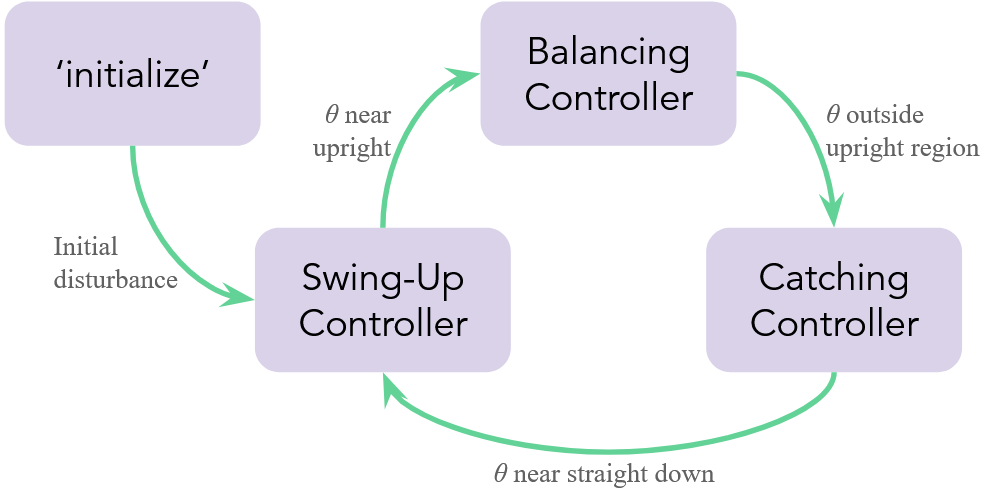
\includegraphics[width=0.6\textwidth]{figures/state_machine.png}
    \caption{State machine for mode switching between controllers.}
    \label{fig:state_machine}
\end{figure}

\section{Closed-Loop Performance}

Closed-loop experiments validated the controllers' performance. The step response showed quick stabilization and effective handling of mode transitions.

\begin{figure}[H]
    \centering
    
\includegraphics[width=0.8\textwidth]{figures/ph.png}
    \caption{Closed-loop step response for cart and pendulum positions.}
    \label{fig:step_response}
\end{figure}

\section{Conclusions and Future Work}
The controllers successfully addressed swing-up, balancing, and catching objectives, validating theoretical designs with robust experimental performance. Further work includes enhancing failure logic and addressing steady-state error.

\bibliographystyle{IEEEtran}
\bibliography{references}

\end{document}
